\chapter{Anwendungsfall und Prototyp}
\label{chapter:prototype}

In den Kapiteln zuvor wurde in das Thema durch Grundlagen und eine Vorstellung der einzelnen Streaming frameworks eingeführt. Das Kapitel \ref{chapter:prototype} beschreibt eine Methode zur Messung der Performance. Es wird zunächst das Messverfahren gezeigt und die Messumgebung beschrieben. Abschließend wird eine Messung durchgeführt und die Messergebnisse vorgestellt.

In der Abbildung \ref{fig:prototypeStreamingGraph} wird ein erster Bildschirmausschnitt aus einer Messung mit Apache Storm über ein Standardtestdatensatz für das Zählen von Worten gezeigt.

\begin{figure}[htb!]
\centering
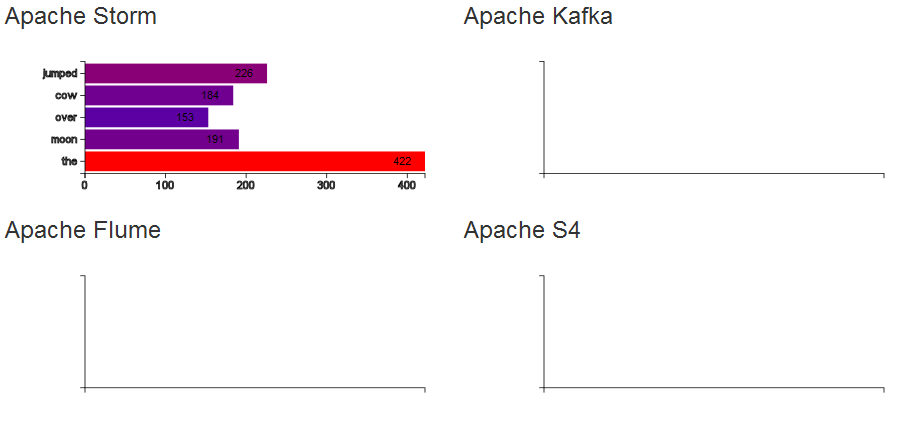
\includegraphics[width=1.0\textwidth]{bilder/PrototypeStreamingGraph.png}
\caption{Prototype Streaming Graph
\label{fig:prototypeStreamingGraph}}
\end{figure}

\begin{figure}
\begin{tikzpicture} 
\begin{axis}[ enlarge x limits=0.03, 
							%title=Messung,
							xlabel=$t$ in Sekunden,
							ylabel=Anzahl Nachrichten,
							axis x line=bottom,
							axis y line=left,
							ymin=0,
							ymax=200,
							width=1\linewidth,
							height=10cm,
							legend entries = {Apache Storm, Apache Kafka, Apache Flume, Apache S4},
							legend style={at={(1,1)},xshift=0.2cm,anchor=north east,nodes=right} ] 
%nur punkte
%\addplot+[only marks, color=blue, mark options={scale=0.08}, mark=*] table [x=Time, y=Mps, col sep=comma,trim cells=true] {anhangMessung/traversedMeasure.log};
%verbundene Punkte
\addplot+ table [x=Time, y=Mps, col sep=comma,trim cells=true] {anhangMessung/traversedMeasureStorm.log};
\addplot+ table [x=Time, y=Mps, col sep=comma,trim cells=true] {anhangMessung/traversedMeasureKafka.log};
\addplot+ table [x=Time, y=Mps, col sep=comma,trim cells=true] {anhangMessung/traversedMeasureFlume.log};
\addplot+ table [x=Time, y=Mps, col sep=comma,trim cells=true] {anhangMessung/traversedMeasureS4.log};
\end{axis} 
\end{tikzpicture}

\caption{Messung Streaming frameworks
\label{fig:messung}}
      \end{figure}
